\documentclass[12pt,letterpaper]{article}
\usepackage{fullpage}
\usepackage[top=2cm, bottom=4.5cm, left=2.5cm, right=2.5cm]{geometry}
\usepackage{amsmath,amsthm,amsfonts,amssymb,amscd}
\usepackage{lastpage}
\usepackage{enumerate}
\usepackage{fancyhdr}
\usepackage{mathrsfs}
\usepackage{xcolor}
\usepackage{graphicx}
\usepackage{listings}
\usepackage{hyperref}
\usepackage{enumitem}
\usepackage{amssymb,amsmath,mathabx, amscd}
\usepackage[pdftex]{graphicx}
\usepackage{enumerate}
\usepackage{tikz, tikz-cd}
\usepackage[margin=.8in]{geometry}
\usepackage{color}
\usepackage{hyperref}
\usepackage{mathrsfs, colonequals}
\usepackage{tikz-3dplot}


\newcommand{\cc}{\mathbb{C}}
\newcommand{\ff}{\mathbb{F}}
\renewcommand{\gg}{\mathbb{G}}
\newcommand{\qq}{\mathbb{Q}}
\newcommand{\rr}{\mathbb{R}}
\newcommand{\zz}{\mathbb{Z}}
\renewcommand{\P}{\mathcal{P}}
\newcommand{\aaa}{\text{ and }}
\newcommand{\oo}{\text{ or }}

\newtheorem{thm}{Theorem}[section]
\newtheorem{ithm}{Theorem}
\newtheorem{icor}[ithm]{Corollary}
\newtheorem{lem}[thm]{Lemma}
\newtheorem{conj}[thm]{Conjecture}
\newtheorem{prop}[thm]{Proposition}
\newtheorem{cor}[thm]{Corollary}
\newtheorem{claim}[thm]{Claim}

\theoremstyle{definition}
\newtheorem{defin}[thm]{Definition}
\newtheorem{example}[thm]{Example}
\newtheorem{assumption}[thm]{Assumption}
\newtheorem{exercise}[thm]{Exercise}
\newtheorem*{question}{Main Question}

\theoremstyle{remark}
\newtheorem{rem}{Remark}

\newcommand{\nul}{\operatorname{null}}
\newcommand{\range}{\operatorname{range}}
\renewcommand{\implies}{\Rightarrow}
\renewcommand{\iff}{\Leftrightarrow}
\newcommand{\defi}[1]{{\color{violet}\textsf{#1}}}
\hypersetup{%
    colorlinks=true,
    linkcolor=blue,
    linkbordercolor={0 0 1}
}

\renewcommand\lstlistingname{Algorithm}
\renewcommand{\qedsymbol}{$\blacksquare$}
\renewcommand\lstlistlistingname{Algorithms}
\def\lstlistingautorefname{Alg.}

\lstdefinestyle{Python}{
    language        = Python,
    frame           = lines,
    basicstyle      = \footnotesize,
    keywordstyle    = \color{blue},
    stringstyle     = \color{green},
    commentstyle    = \color{red}\ttfamily
}

\setlength{\parindent}{0.0in}
\setlength{\parskip}{0.05in}

% Edit these as appropriate
\newcommand\course{MATH 540}

\pagestyle{fancyplain}
\headheight 35pt
\lhead{\NetIDa}
%\lhead{\NetIDa\\\NetIDb}                 % <-- Comment this line out for problem sets (make sure you are person #1)
\chead{\textbf{\Large PSET 7 \hwnumber}}
\lhead{\course}
\rhead{\today}
\cfoot{}
\rfoot{\small\thepage}
\headsep 1.5em

\begin{document}

    \section*{Problem 1}

    Let maps $T\in \mathcal{L}(U,V), S \in \mathcal{L}(V,W)$ be invertible, show that $ST \in \mathcal{L}(U,W)$ is invertible and $(ST)^{-1} = T^{-1}S^{-1}$. Because $T$ is invertible from $U$ to $V$, we see that $dimU=dimV$. Because $S$ is invertible from $V$ to $W$, we also have $dimV=dimW$. Therefore, $dimV=dimW$. Because dimension is sufficient to show isomorphism, we see that $ST$ is invertible because dimension is preserved. Now, we can write $ST(ST)^{-1}=I$. Now we must evaluate $ST(ST)^{-1}$ to see if it gives the identity. Using composition of linear maps, we can rewrite this as $ST(T^{-1}S^{-1})$. Using linearity, we see that $S(TT^{-1})S^{-1}$. Because T is invertible, we have $SIS^{-1}$. Because I is the identity, we have $SS^{-1}$, which is equal to $I$ because $S$ is invertible. Therefore, $(ST)^{-1}=T^{-1}S^{-1}$.

    \section*{Problem 2}

    Let $V$ be finite-dimensional and $S,T \in \mathcal{L}(V)$. First assume that $ST=I$. Given vector $v_1,v_2 \in V$ such that $T(v_1)=v_2$, we can multiply both sides by $S$ to get $ST(v_1)=S(v_2)$. Now, we see that $ST$ is defined as the identity, so we can rewrite this as $v_1=S(v_2)$. Now, multiplying both sides by T, we see that $T(v_1)=TS(v_2)$. substituting and using properties of linearity, we now have $v_2=(TS)v_2$. Therefore, $TS=I$. Now assume that $TS=I$. Given any vectors $v_1,v_2 \in V$ such that $S(v_1)=v_2$, we can write $TS(v_1)=T(v_2)$. Because $TS$ is defined as the identity, we have $v_1=T(v_2)$. Multiplying both sides by $S$, we get $S(v_1)=ST(v_2)$. Substituting and using properties of linearity, we see that $v_2=(ST)v_2$. Therefore $ST=I$. Because this holds both ways, $ST=I$ if and only if $TS=I$

    \section*{Problem 3}
    \begin{enumerate}[label=\alph*]
        \item Given any field $\ff$, show that $\ff^{n_1} \times \ff^{n_2}$ is isomorphic to $\ff^{n_1+n_2}$. According to Axler 3.76, we can find the dimension of the Cartesian product by summing each element's dimension. In this case, we get $dim \ff^{n_1} \times \ff^{n_2} = dim \ff^{n_1} + dim \ff^{n_2}=n_1+n_2$. Because the dimension of $\ff^{n_1+n_2}$ is simply $n_1+n_2$, we see that $\ff^{n_1} \times \ff^{n_2}$ is isomorphic to $\ff^{n_1+n_2}$.
        \item Given a linear map $T:U \times V \to W$, show that $T((u,v)) = T((u,0)) + T((0,v))$. To evaluate $T((u,0)) + T((0,v))$, we must use properties of vector spaces. Adding these together, we get $T((u,0)) + T((0,v))= T((u+0),(v+0))$, which simplifies to  $T((u,0)) + T((0,v))= T((u,v))$
        \item For all $T \in \mathcal{L}(U \times V, W)$, define $T: U \times V \to W$ such that for all $u \in U, v \in V, T_1(u,v) =(u,0)$ and $T_2(u,v)=(0,v)$. Now define map $S : \mathcal{L}(U \times V, W) \to \mathcal{L}(U,W) \times \mathcal{L}(V,W)$ such that $S(T)=(T_1+T_2)$ (part b). To see if this is an isomorphism, we must construct an inverse map. We can define $G:\mathcal{L}(U,W) \times \mathcal{L}(V,W) \to \mathcal{L}(U \times V, W)$
    \end{enumerate}

    \section*{Problem 4}
    Given nonempty subset $A$ of $V$, show that it is an affine subset of $V$ if and only if $\lambda v + (1- \lambda)w \in A$ for all $v,w \in A$ and for all $\lambda \in \ff$. Assume A is an affine subset of V, it can be expressed in the form $A=a+U$ where $a \in V$ and $U$ is a subspace of $V$. Now, we can write $v = a + u_1$ and $w = a + u_2$ where $u_1,u_2 \in U$. Substituting this into the original expression, we have $\lambda(a + u_1) + (1-\lambda)(a + u_2)$, which we can see is contained within the subset $a + U$, which we defined as $A$. Now assume that $\lambda v + (1- \lambda)w \in A$ for all $v,w \in A$ and for all $\lambda \in \ff$. We must show that $A = a + U$ is an affine subset of V. To do this, we can show $U = A - a$ is a subspace of V. If this is true, then $A$ is an affine subset of $V$ because it can be written in the form $A = a + (A - a)$. To show this, we can write $A-a = \{x-a:x \in A \}$. Following our assumption, we can substitute and see that for some $x-a \in A-a$, and $\lambda \in \ff$, we have $\lambda (x) + (1-\lambda)(a) \in A$. Simplifying, we get $\lambda(x-a)$, which shows that scalar multuplication is closed under $U$. Now we must show that $U$ is closed under addition. Given any $(x-a) + (y-a)$, we can write this as $2(\frac{x}{2} + \frac{y}{2} - a)$ Because $U$ is closed under scalar multiplication, we see that $U$ is also closed under addition. Therefore, $U$ is a subspace of $V$. As stated before, this shows that $A$ is an affine subset.

    \section*{Problem 5}
    \begin{enumerate}[label=\alph*]
        \item
        \begin{enumerate}[label=\roman*]
                  \item 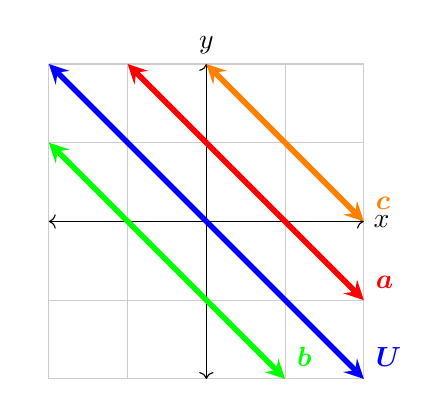
\begin{tikzpicture}
                            \draw[thin,gray!40] (-2,-2) grid (2,2);
                            \draw[<->] (-2,0)--(2,0) node[right]{$x$};
                            \draw[<->] (0,-2)--(0,2) node[above]{$y$};
                            \draw[line width=2pt,blue,-stealth](0,0)--(2,-2) node[anchor=south west]{$\boldsymbol{U}$};
                            \draw[line width=2pt,blue,-stealth](0,0)--(-2,2) node[anchor=north east]{$\boldsymbol{}$};
                            \draw[line width=2pt,red,-stealth](1,0)--(2,-1) node[anchor=south west]{$\boldsymbol{a}$};
                            \draw[line width=2pt,red,-stealth](1,0)--(-1,2) node[anchor=north east]{$\boldsymbol{}$};
                            \draw[line width=2pt,green,-stealth](-1,0)--(1,-2) node[anchor=south west]{$\boldsymbol{b}$};
                            \draw[line width=2pt,green,-stealth](-1,0)--(-2,1) node[anchor=north east]{$\boldsymbol{}$};
                            \draw[line width=2pt,orange,-stealth](1,1)--(2,0) node[anchor=south west]{$\boldsymbol{c}$};
                            \draw[line width=2pt,orange,-stealth](1,1)--(0,2) node[anchor=north east]{$\boldsymbol{}$};
                  \end{tikzpicture}\\
                  $a = U + (1,0), b=U+(-1,0),c=U+(2,0)$
                  \item Let $W = (x,0), x \in \rr$. Let $\phi : V/U \to W$ be defined by $\phi (v + U: v \in V) = (v, 0)$. This map takes the vector that $U$ is translated by and puts it on the x-axis. To show that this is isomorphic, we must show that the dimensions are equal. Using the rank-nullity theormen, we see that $dim(W) = rank(W) + nullity(W) = 1 + 0 = 1$. We also see that $dim(V/U) = dim(V) - dim(U) = 2 - 1 = 1$. Since the dimensions are equal, they are isomorphic. Hence, this map is an isomorphism.
        \end{enumerate}
    \end{enumerate}
    \section*{Problem 6}
    begin problem

\end{document}